\documentclass{beamer}
\usetheme[deutsch]{KIT}

\usepackage[utf8]{inputenc}
\usepackage[T1]{fontenc}
\usepackage{babel}
\usepackage{tikz,calc,ifthen}
\usepackage{mathtools}
\usepackage[normalem]{ulem}
\usepackage{graphicx}

\usepackage{xcolor}
\definecolor{darkblue}{RGB}{0,0,200}
\definecolor{darkred}{RGB}{200,0,0}
\definecolor{darkgreen}{RGB}{0,160,0}
\definecolor{darkbrown}{RGB}{160,30,70}
\definecolor{darkorange}{RGB}{255, 102, 0}
\definecolor{darkturqoise}{RGB}{0,170,136}
\definecolor{darkdarkblue}{RGB}{212,0,170}

\usetikzlibrary{positioning,calc,arrows,shapes}
\tikzset{
  every node/.style={transform shape},
  auto,
  block/.style={align=center,rectangle,draw,minimum height=20pt,minimum width=30pt},
  >=triangle 60,
  alt/.code args={<#1>#2#3}{%
      \alt<#1>{\pgfkeysalso{#2}}{\pgfkeysalso{#3}}
  },
  beameralert/.style={alt=<#1>{color=green!80!black}{}},
  mythick/.style={line width=1.4pt}
}

\newcommand*{\maxwidthofm}[2]{\maxof{\widthof{$#1$}}{\widthof{$#2$}}}
\newcommand<>*{\robustaltm}[2]{
  \alt#3
  {\mathmakebox[\maxwidthofm{#1}{#2}]{#1}\vphantom{#1#2}}
    {\mathmakebox[\maxwidthofm{#1}{#2}]{#2}\vphantom{#1#2}}
}

\newcommand<>*{\nodealert}[1]{\only#2{\draw[overlay,mythick,color=green!80!black]
(#1.north west) rectangle (#1.south east)}}

\title{Invasives Rust}
\author{Hermann Heinz Erich Krumrey}
\subtitle{\insertauthor}
\institute[IPD]{Lehrstuhl Programmierparadigmen, IPD Snelting}
\date{29.10.2013}
\KITtitleimage{images/cover.png}

\begin{document}

\begin{frame}
  \maketitle
\end{frame}

%-----------------------------------------------------------------------------------------------------------------------


\begin{frame}{Motivation}

  \begin{center}
    \only<1>{
\includegraphics[width=0.6\textwidth]{images/example-base.pdf}}
    \only<2>{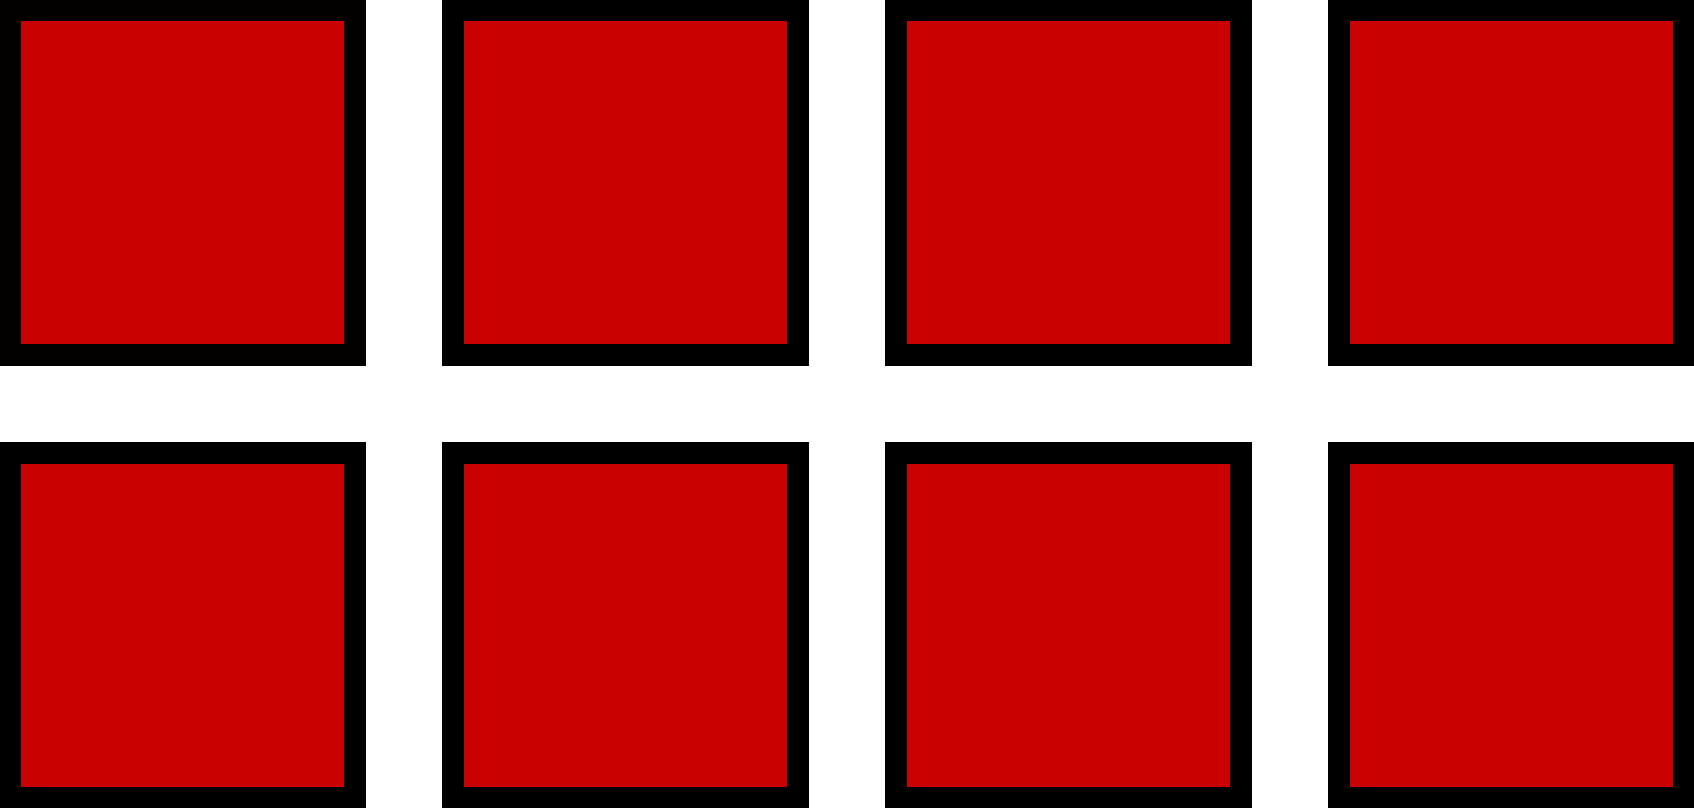
\includegraphics[width=0.6\textwidth]{images/example-step-one.pdf}}
    \only<3>{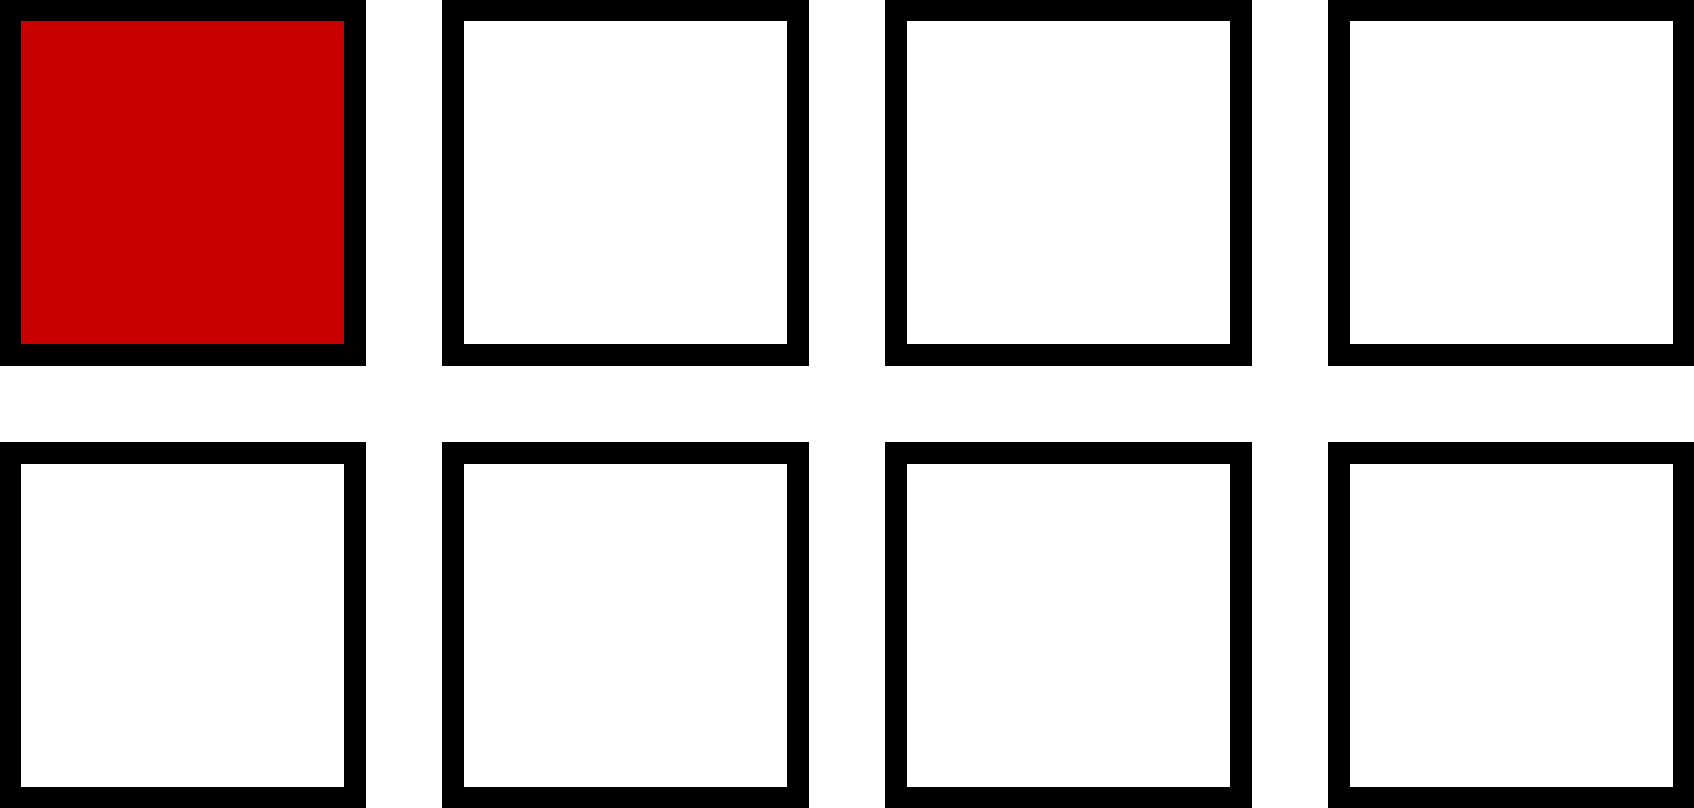
\includegraphics[width=0.6\textwidth]{images/example-step-two.pdf}}
    \only<4>{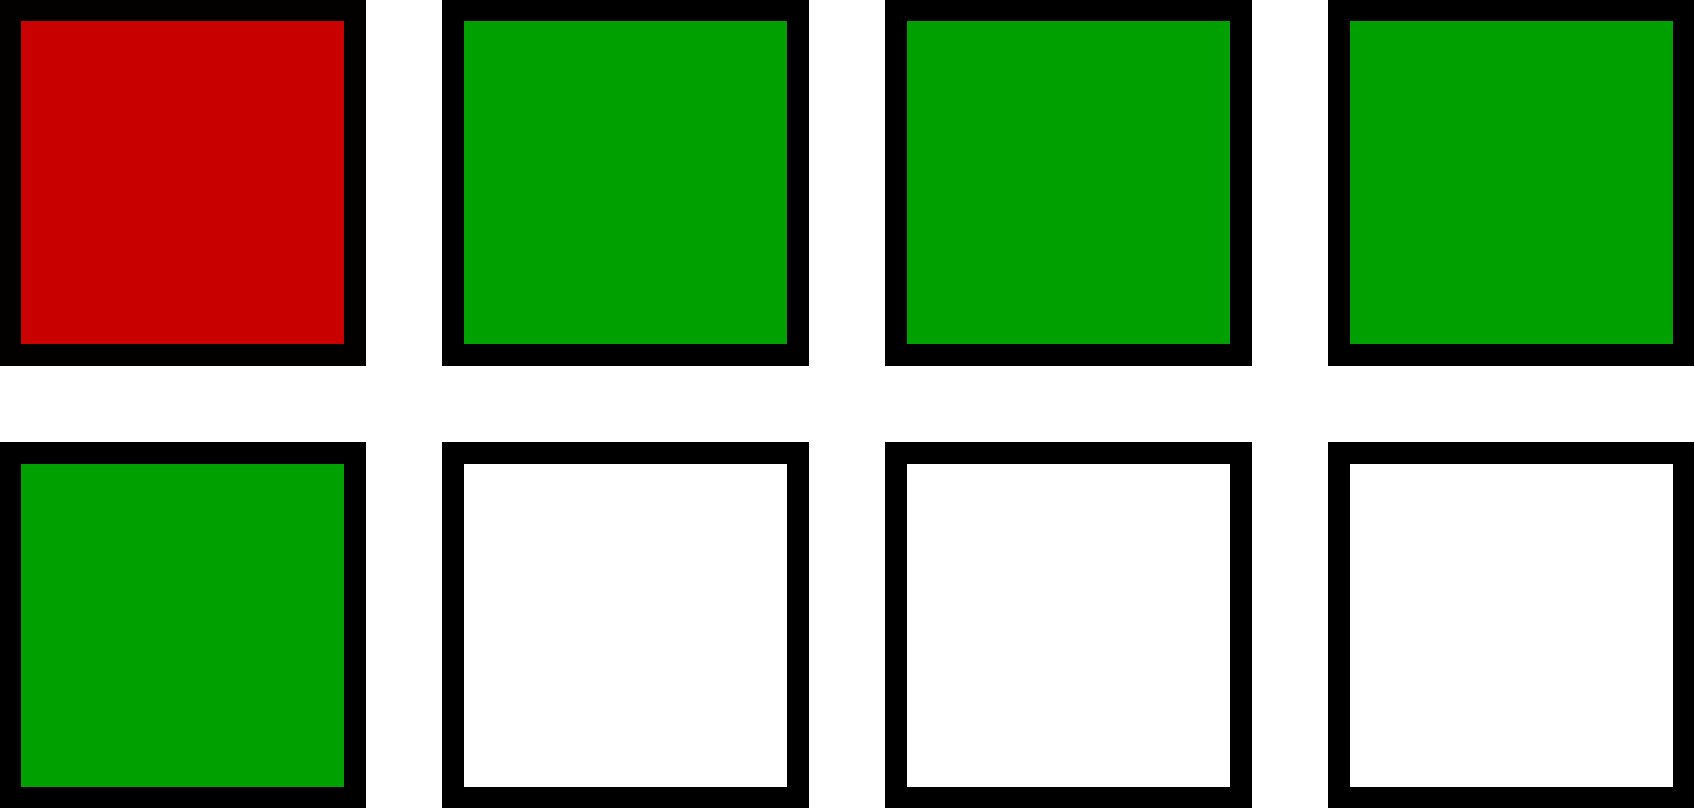
\includegraphics[width=0.6\textwidth]{images/example-step-three.pdf}}
    \only<5>{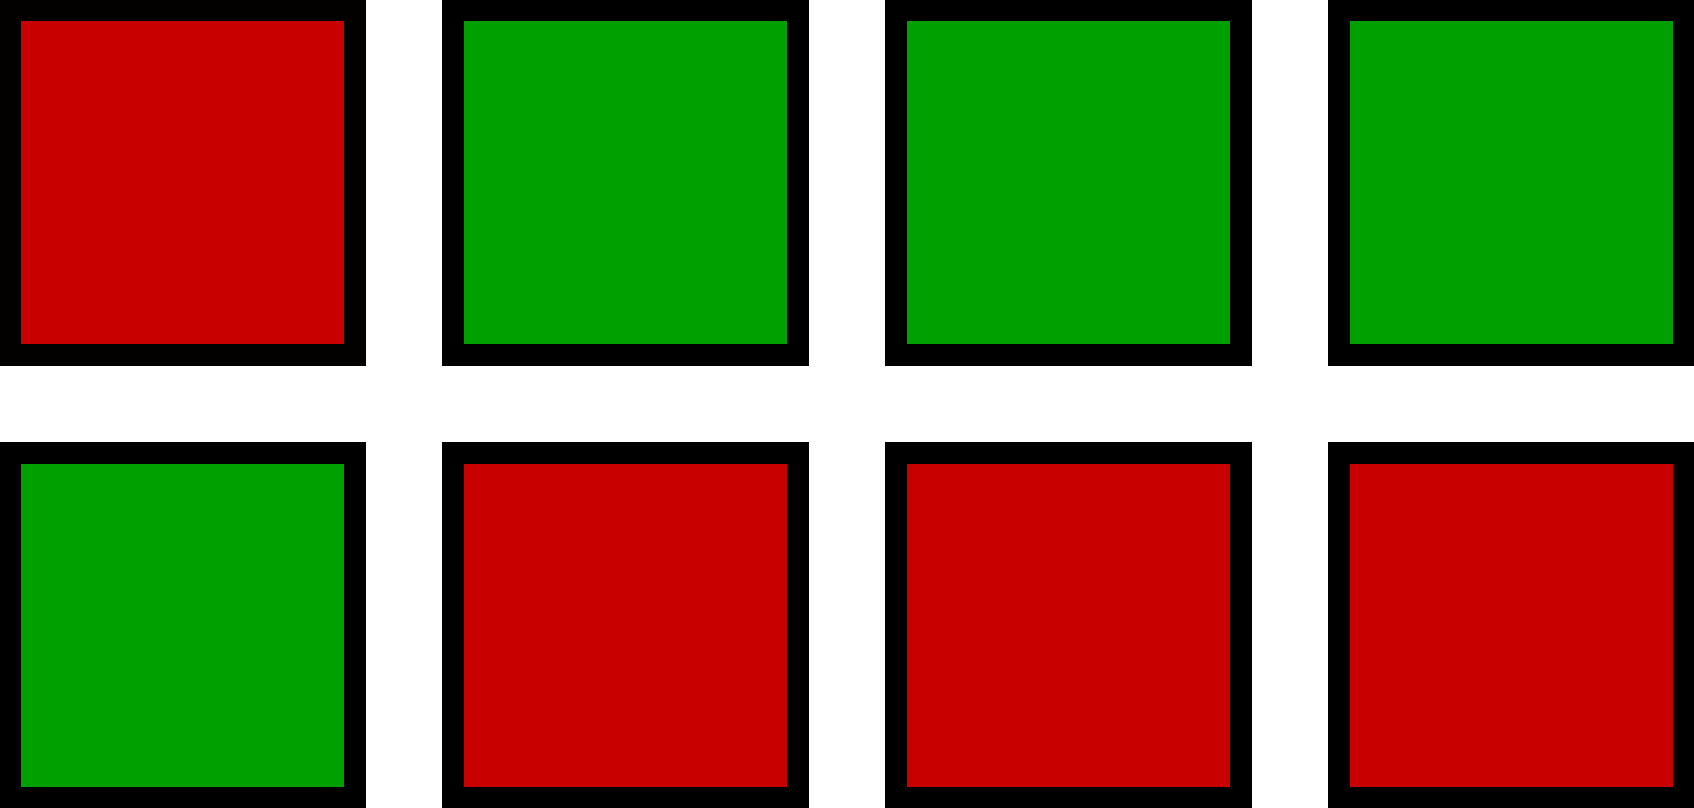
\includegraphics[width=0.6\textwidth]{images/example-step-four.pdf}}

  \end{center}

  \begin{enumerate}
    \item<2-> \textcolor{darkred}{Programm 1} beginnt Ausführung auf 8 Recheneinheiten
    \item<3-> \textcolor{darkred}{Programm 1} sendet Ergebnisse über das Netzwerk
    \item<4-> \textcolor{darkgreen}{Programm 2} beginnt Ausführung auf 4 Recheneinheiten
    \item<5-> \textcolor{darkred}{Programm 1} führt wieder Berechnungen aus, jetzt auf 4 Recheneinheiten

  \end{enumerate}
  
\end{frame}

\begin{frame}{Invasives Rechnen}

\begin{center}
  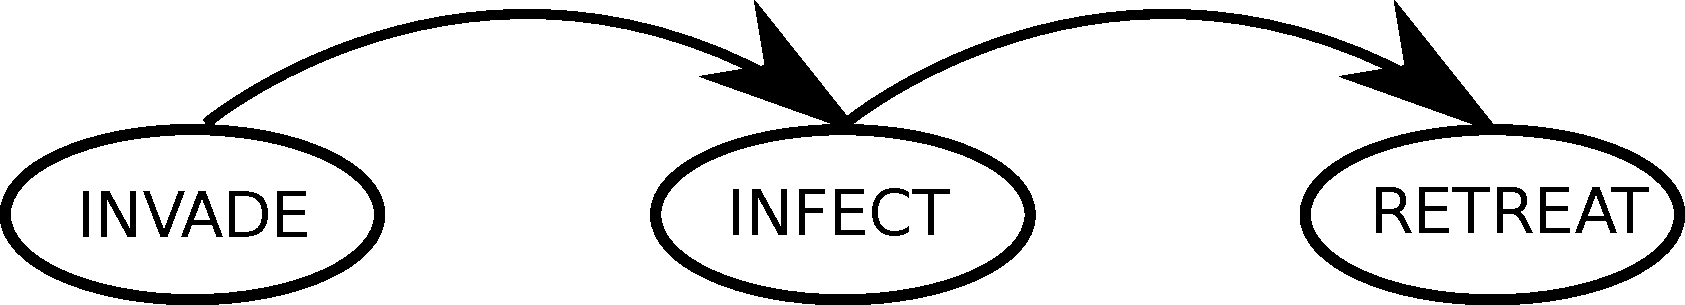
\includegraphics[width=0.7\textwidth]{images/invadeInfectRetreat.pdf}
\end{center}

  \begin{itemize}
    \item Ressourcenbewusstes Programmieren
    \item 3 Phasen:
      \begin{enumerate}
        \item Invade - Ressourcen reservieren
        \item Infect - Ressourcen nutzen
        \item Retreat - Ressourcen freigeben 
      \end{enumerate}
    \item OctoPOS und iRTSS bieten Software-Grundlage
    \item Angepasste Hardware um invasive Grundfunktionen zu unterstützen
  \end{itemize}
  
\end{frame}

\begin{frame}{SPARC LEON}

    \begin{itemize}
      \item SPARC
        \begin{itemize}
          \item Skalierbare Prozessorarchitektur
        \end{itemize}
      \item SPARC-V8
        \begin{itemize}
          \item Basierend auf SPARC
          \item 32-bit Architektur
        \end{itemize}
      \item LEON
        \begin{itemize}
          \item SPARC-V8 basierte Prozessorfamilie
          \item Konfigurierbare, Open-Source VHDL Designs
          \item Geeignet für den Einsatz in angepassten ASICs, SOCS und FPGAs
        \end{itemize}
    \end{itemize}

\end{frame}

\begin{frame}{Rust - Motivation}
    \begin{itemize}
      \item Sichere Speicherzugriffe
      \item Effiziente und sicherere Parallelberechnung
      \item Konzeptionell an C-artige Sprachen angelehnt
      \item Höhere Abstraktionen, um den Einstieg zu erleichtern
      \item Speichersicherheit und Abstraktionen sollen nicht
            auf Kosten der Leistung erreicht werden
    \end{itemize}
\end{frame}

\begin{frame}{Rust - Ownership}
    
    Das zentrale Alleinstellungsmerkmal der Programmiersprache

    \begin{itemize}
      \item Jeder Speicherbereich wird nur einer einzigen Variable zur Verfügung gestellt
      \item Beim Verlassen des Geltungsbereichs wird der Speicherbereich freigegeben
    \end{itemize}

\end{frame}

\begin{frame}{Rust - Move-Semantik und Referenzen}
    

    \begin{itemize}
      \item Move-Semantik
        \begin{itemize}
          \item Move
        \end{itemize}
      \item Referenzen
        \begin{itemize}
          \item Ref
          \item mut Ref
        \end{itemize}
    \end{itemize}

\end{frame}

\begin{frame}{Rust - Ownership - Beispiel}
  Beispiel aus thesis, Colour-coded, step-by step
\end{frame}

\begin{frame}{Rust - SPARC}


    nostd
    JSON
    libcore
    Cargo
\end{frame}

\begin{frame}{octorust}

  \begin{itemize}
    \item Hilfsprogramm zum Kompilieren von invasiven Rust-Programmen
    \item Kompilierung von \textbf{.rs}-Dateien und Cargo-Projekten
    \item Unterstützung von SPARC-V8
    \item Automatische Verlinkung mit iRTSS/OctoPOS
    \item ca. 650 Zeilen Code (Python)
  \end{itemize}

\end{frame}

\begin{frame}{octolib}
    \begin{itemize}
      \item Direkte C-Rust Bindings
      \item Rust-spezifische Änderungen
      \item ca. 750 Zeilen Code (Rust)
    \end{itemize}
\end{frame}

\begin{frame}{octolib - Rust Bindings}
  \begin{itemize}
    \item Beispiel C Funktion zu Rust Funktion
  \end{itemize}
\end{frame}

\begin{frame}{octolib - Rust Improvements}
    \begin{itemize}
      \item AgentClaim
      \item Closures
    \end{itemize}
\end{frame}

\begin{frame}{Evaluation}
    \begin{itemize}
      \item temci
      \item 50-mal
      \item Intel i5...
      \item Benchmarks
        \begin{itemize}
          \item Kompilierungsdauer
          \item Parallele Primzahlenberechnung
          \item Allokation von Objekten
        \end{itemize}
    \end{itemize}
\end{frame}

\begin{frame}{Kompilierungsdauer}
  \begin{center}
    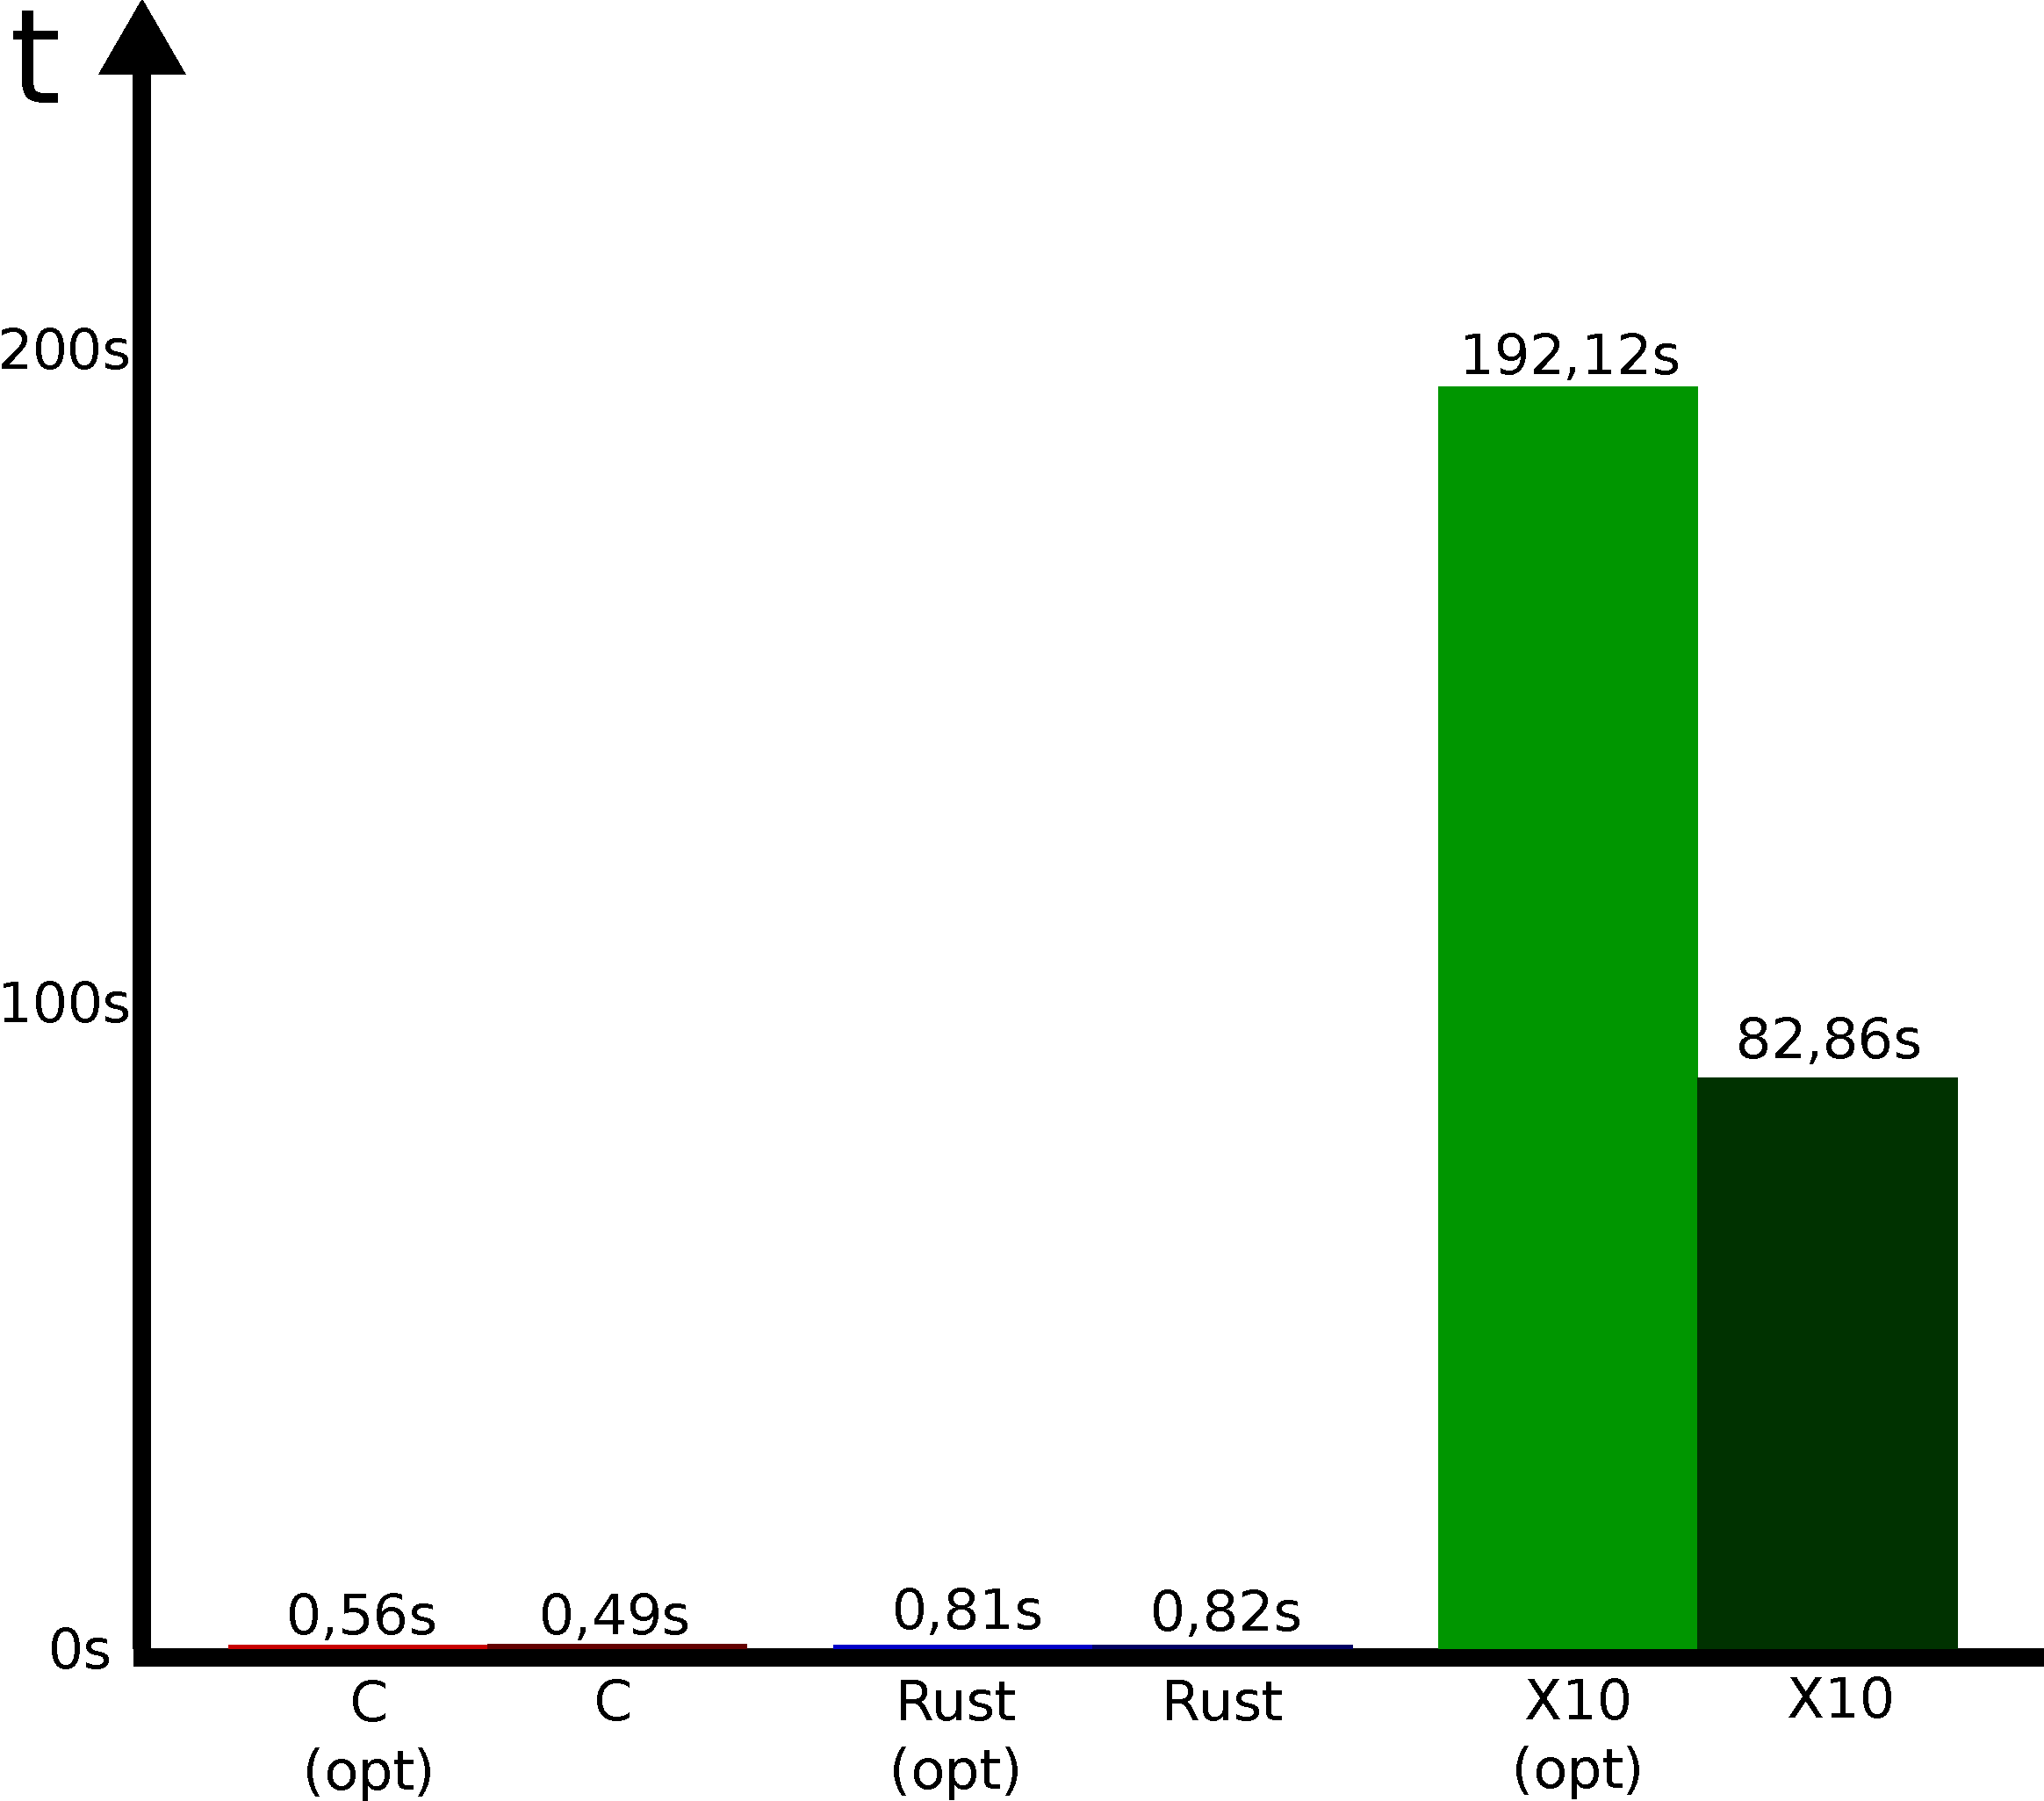
\includegraphics[width=0.6\textwidth]{images/compile-eval.pdf}
  \end{center}
  \begin{itemize}
    \item X10 langsam
  \end{itemize}
\end{frame}

\begin{frame}{Parallele Primzahlenberechnung}
  \begin{center}
    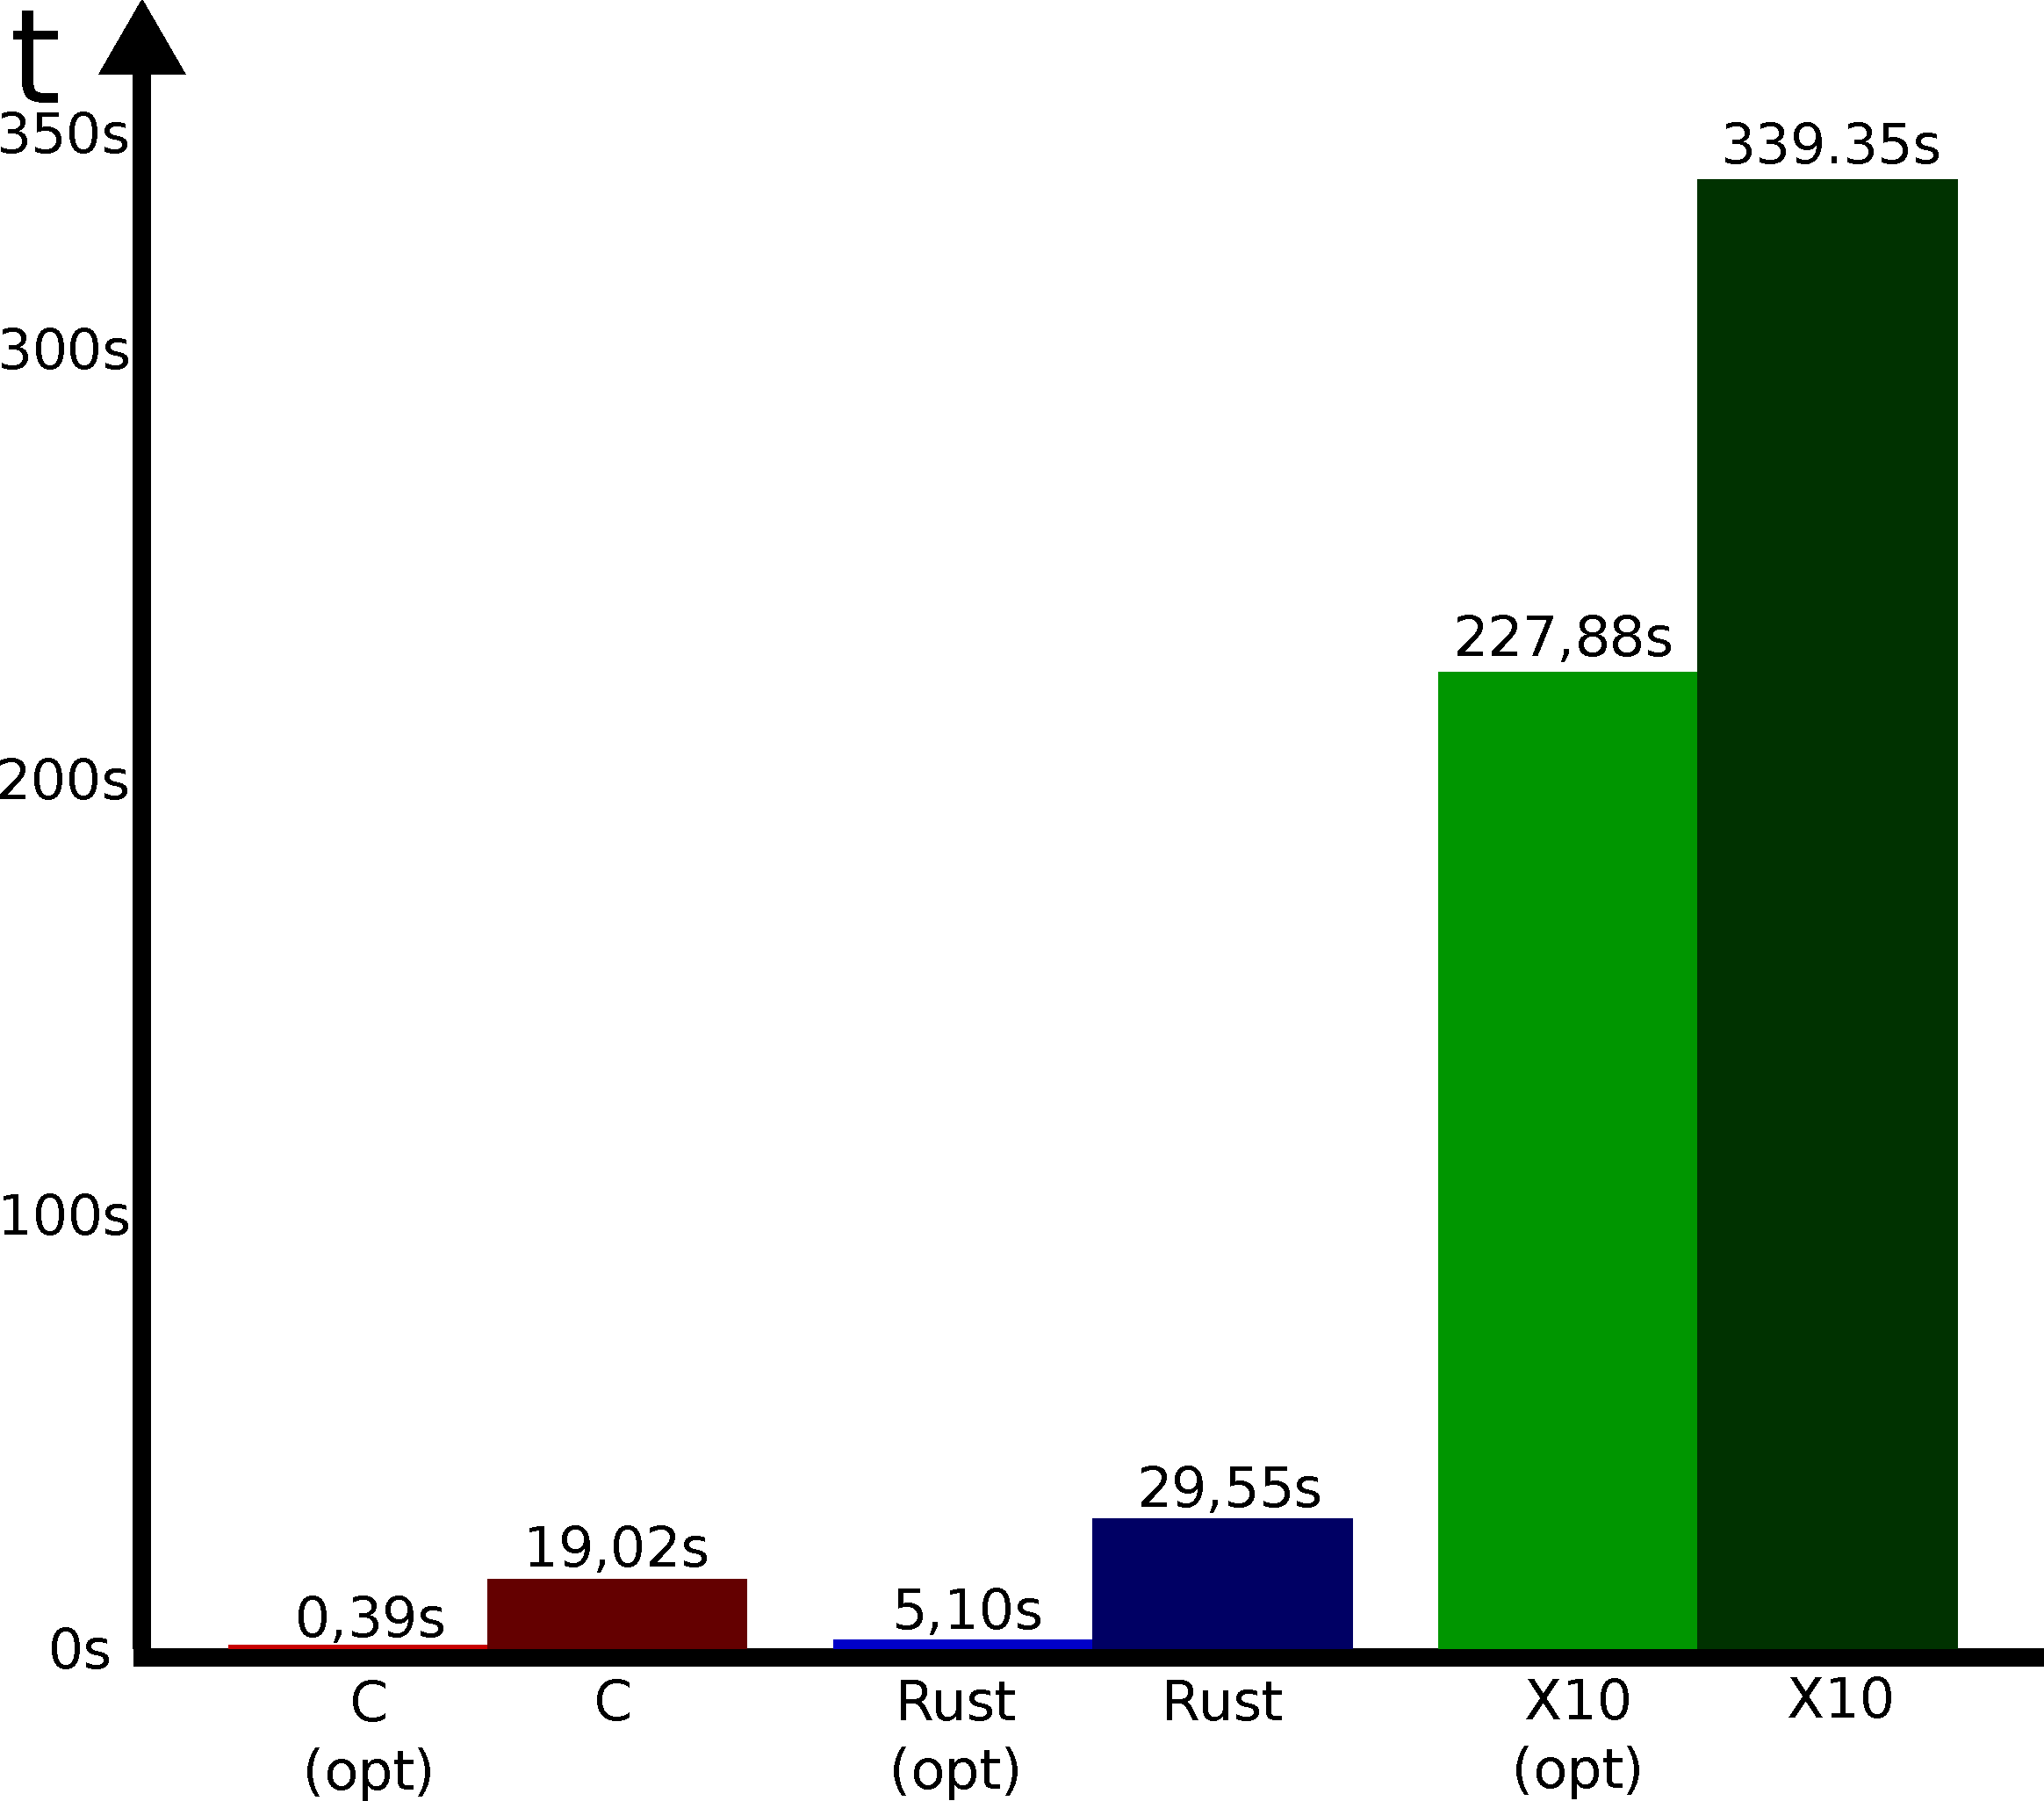
\includegraphics[width=0.6\textwidth]{images/primes-eval.pdf}
  \end{center}
  \begin{itemize}
    \item Rust langsam
  \end{itemize}
\end{frame}

\begin{frame}{Allokation von Objekten}
  \begin{center}
    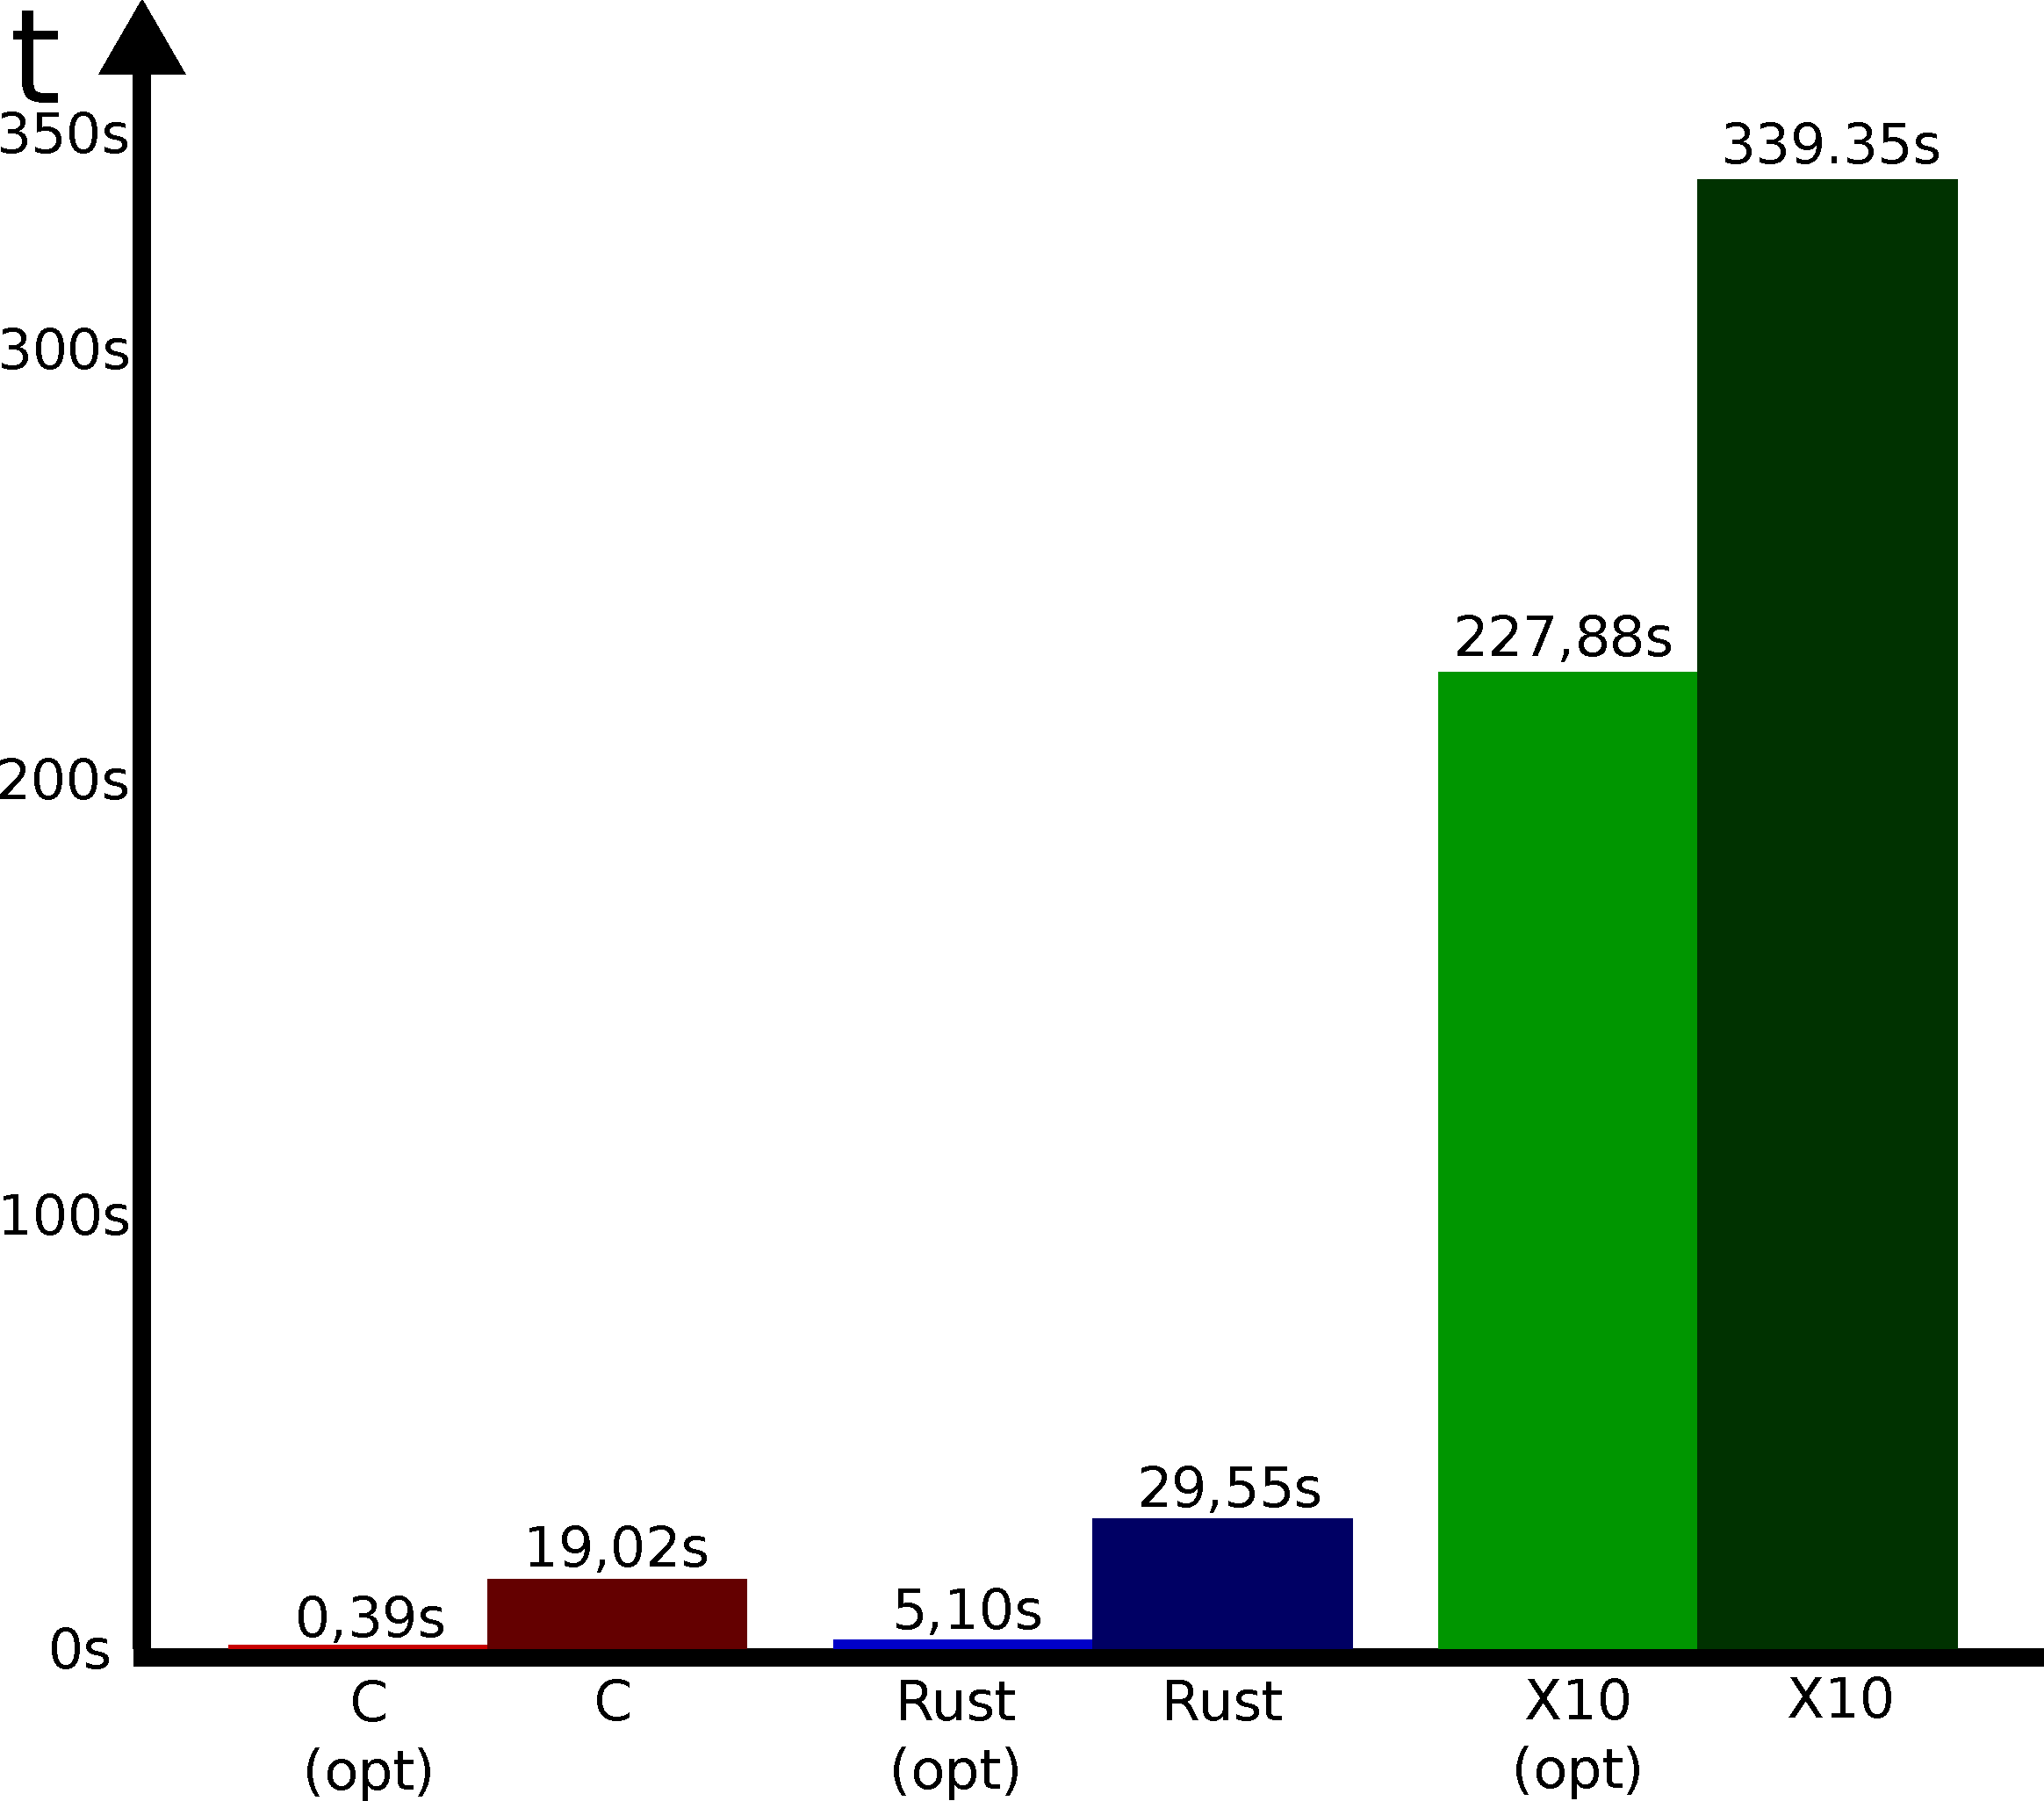
\includegraphics[width=0.6\textwidth]{images/garbage-eval.pdf}
  \end{center}
  \begin{itemize}
    \item X10 langsam
  \end{itemize}
\end{frame}


\begin{frame}{Zusammenfassung und Fazit}
\end{frame}

\begin{frame}{Fragen?}
    4 Wichtigste Folien:
    
    invasive computing
    
    ownership - beispiel
    
    structs etc
    
    octolib - improvements
\end{frame}

\end{document}
